\chapter{Plan del proyecto}

Una vez definidos los requisitos del sistema, es necesario establecer una estrategia de ejecución
detallada antes de la fase de desarrollo. El objetivo de este capítulo es fijar los recursos
necesarios, organizar las tareas en el tiempo mediante una planificación en forma de calendario,
analizar las tecnologías elegidas para cada componente y calcular el coste final estimado del
proyecto.

El desarrollo se estructura de forma ágil, basada en \textit{sprints} (ciclos cortos de trabajo),
con el objetivo de ir creando pequeñas versiones funcionales del proyecto de manera continua. Esto
aumenta la claridad del desarrollo y la capacidad de adaptación ante cambios o errores detectados a
lo largo del proceso, y permite al director validar los avances \textit{sprint} a \textit{sprint}.

\section{Recursos}

Es fundamental establecer con qué medios se cuenta para realizar el proyecto. Se dividen en dos
grupos: los recursos humanos y los recursos materiales. Como es lógico en un TFG, el alumno asume
todos los roles, pero para poder hacer una estimación realista de costes se toma como referencia el
mercado laboral actual de España, simulando que el proyecto lo llevan a cabo varios profesionales.

\subsection{Recursos humanos}

Dependiendo de la fase del proyecto en la que se esté, hace falta un perfil técnico u otro. Teniendo
esto en cuenta, se han definido los cinco roles que recoge la tabla~\ref{tab:salarios}, con una
estimación de su salario medio.

\begin{table}[H]
	\centering
	\caption{Salario medio del personal.}
	\label{tab:salarios}
	\begin{tabularx}{0.75\textwidth}{X r r}
		\toprule
		\textbf{Rol} & \textbf{Salario anual bruto} & \textbf{Salario por hora} \\
		\midrule
		Analista                  & 31.500\,\euro{} & 16,15\,\euro{} \\
		Ingeniero de Datos        & 30.000\,\euro{} & 15,38\,\euro{} \\
		Ingeniero de Requisitos   & 35.000\,\euro{} & 17,95\,\euro{} \\
		Ingeniero de Software     & 35.000\,\euro{} & 17,95\,\euro{} \\
		Programador               & 28.500\,\euro{} & 14,62\,\euro{} \\
		\bottomrule
	\end{tabularx}
\end{table}

Estos datos son una aproximación basada en ofertas reales del sector~\cite{salarios}, y pueden variar
en función del momento en el que se consulten o del nivel y experiencia de los profesionales. Estos
cinco roles intervienen en distintas fases del proyecto: en las fases iniciales de ingeniería
participan el Analista y el Ingeniero de Requisitos, mientras que en los sprints de desarrollo lo
hacen el Ingeniero de Datos, el Ingeniero de Software y el Programador. Al ser Brain Viz una
aplicación web de visualización 3D, dentro de cada sprint las tareas se dividen entre \textit{backend}
y \textit{frontend}, tal y como resume la tabla~\ref{tab:secciones}.

\begin{table}[H]
	\centering
	\caption{Secciones típicas dentro de un sprint de desarrollo y rol encargado.}
	\label{tab:secciones}
	\begin{tabularx}{\textwidth}{X >{\centering\arraybackslash}p{1.8cm} l}
		\toprule
		\textbf{Sección} & \textbf{Capa} & \textbf{Encargado} \\
		\midrule
		Procesamiento de datos y algoritmos        & Backend  & Ingeniero de Datos \\
		Diseñar la API y su comunicación           & Backend  & Ingeniero de Software \\
		Diseñar el entorno y la visualización 3D   & Frontend & Ingeniero de Software \\
		Programación e integración del código      & Ambas    & Programador \\
		Pruebas de software y validación           & Ambas    & Ingeniero de Software \\
		\bottomrule
	\end{tabularx}
\end{table}

\subsection{Recursos materiales}

Para sacar adelante la aplicación también es fundamental contar con las herramientas adecuadas,
además del personal técnico. Para estimar el coste del software y del hardware se toma como
referencia lo que marca la Ley del Impuesto sobre Sociedades, que permite estimar una vida útil de 6
años (2190 días) para los productos software y de 8 años (2920 días) para el hardware; el coste
diario es la parte proporcional (amortización) que corresponde al periodo de uso del proyecto. Las
tablas~\ref{tab:software} y~\ref{tab:hardware} recogen, respectivamente, los productos software y
hardware utilizados. Una ventaja importante es que la mayoría de las tecnologías empleadas en el
desarrollo (Docker, Python, Flask, NetworkX, React, Three.js o VS~Code, entre otras) son
\textbf{gratuitas o de código abierto}, por lo que no suponen coste alguno.

\begin{table}[H]
	\centering
	\caption{Productos software utilizados.}
	\label{tab:software}
	\begin{tabularx}{\textwidth}{X r c r}
		\toprule
		\textbf{Licencias} & \textbf{Coste total} & \textbf{Amortización} & \textbf{Coste diario} \\
		\midrule
		Microsoft Windows 11 Pro               & 145,00\,\euro{} & 2190 días & 0,066\,\euro{}/día \\
		Microsoft Office 2024                   & 299,00\,\euro{} & 2190 días & 0,137\,\euro{}/día \\
		VS Code y otras tecnologías gratuitas  & 0,00\,\euro{}   & 2190 días & 0,000\,\euro{}/día \\
		\midrule
		\multicolumn{3}{r}{\textbf{Total}} & \textbf{0,203\,\euro{}/día} \\
		\bottomrule
	\end{tabularx}
\end{table}

\begin{table}[H]
	\centering
	\caption{Productos hardware utilizados.}
	\label{tab:hardware}
	\begin{tabularx}{\textwidth}{X l r c r}
		\toprule
		\textbf{Producto} & \textbf{Tipo} & \textbf{Coste total} & \textbf{Amortización} & \textbf{Coste diario} \\
		\midrule
		ASUS Zenbook 14         & Portátil & 1.099,00\,\euro{} & 2920 días & 0,38\,\euro{}/día \\
		HP OMEN 24 180Hz        & Monitor  & 169,00\,\euro{}   & 2920 días & 0,06\,\euro{}/día \\
		Logitech G203           & Ratón    & 29,99\,\euro{}    & 2920 días & 0,01\,\euro{}/día \\
		Teclado inalámbrico TKL & Teclado  & 69,99\,\euro{}    & 2920 días & 0,02\,\euro{}/día \\
		\midrule
		\multicolumn{4}{r}{\textbf{Total}} & \textbf{0,47\,\euro{}/día} \\
		\bottomrule
	\end{tabularx}
\end{table}

Además de los equipos, el proyecto requiere \textbf{desplegar la aplicación en un servidor público}
para que el director pueda validar cada sprint y, más adelante, el tribunal pueda probarla con
facilidad. Para ello se contempla un servidor virtual (VPS) de bajo coste, estimado en
6,00\,\euro{}/mes.

\section{Planificación temporal}

Para organizar la planificación en forma de calendario se toman jornadas laborales estándar de 8
horas. El desarrollo se divide en cuatro \textit{sprints}, que se corresponden con los cuatro niveles
de prioridad de los requisitos funcionales definidos en el capítulo de requisitos; la asignación
concreta de requisitos a cada sprint se detalló en la tabla~\ref{tab:validacion} de dicho capítulo.
La tabla~\ref{tab:estimacion-sprint} muestra la estimación de días laborables que llevará completar
cada sprint.

\begin{table}[H]
	\centering
	\caption{Estimación temporal por sprint.}
	\label{tab:estimacion-sprint}
	\begin{tabularx}{0.7\textwidth}{>{\centering\arraybackslash}X >{\centering\arraybackslash}X}
		\toprule
		\textbf{Sprint} & \textbf{Estimación temporal} \\
		\midrule
		Sprint 1 & 8 días \\
		Sprint 2 & 7 días \\
		Sprint 3 & 7 días \\
		Sprint 4 & 5 días \\
		\bottomrule
	\end{tabularx}
\end{table}

Además del desarrollo de los \textit{sprints}, el proyecto incluye tareas previas de ingeniería
(análisis de requisitos, casos de uso, planificación y estudio de tecnologías) y la redacción de la
memoria, que se realiza en paralelo al desarrollo y a la que se dedican además algunos días finales
para rematarla y preparar la presentación. La tabla~\ref{tab:tareas} enumera todas las tareas del
proyecto con su responsable y su estimación temporal, e incluye una fila final con el total de días
de trabajo.

\begin{table}[H]
	\centering
	\caption{Tareas del proyecto y estimación temporal.}
	\label{tab:tareas}
	\begin{tabularx}{\textwidth}{>{\centering\arraybackslash}p{1cm} >{\raggedright\arraybackslash}X >{\raggedright\arraybackslash}p{4.2cm} >{\centering\arraybackslash}p{2.1cm}}
		\toprule
		\textbf{N.º} & \textbf{Tarea} & \textbf{Encargado} & \textbf{Estimación} \\
		\midrule
		1 & Análisis de requisitos       & Ingeniero de Requisitos & 3 días \\
		2 & Análisis de casos de uso     & Ingeniero de Requisitos & 2 días \\
		3 & Planificación del proyecto   & Analista                & 2 días \\
		4 & Estudio de tecnologías       & Analista                & 2 días \\
		5 & Sprint 1                     & Equipo de desarrollo    & 8 días \\
		6 & Sprint 2                     & Equipo de desarrollo    & 7 días \\
		7 & Sprint 3                     & Equipo de desarrollo    & 7 días \\
		8 & Sprint 4                     & Equipo de desarrollo    & 5 días \\
		9 & Redacción de la memoria y preparación de la presentación & Analista & 2 días \\
		\midrule
		\multicolumn{3}{r}{\textbf{Total}} & \textbf{38 días} \\
		\bottomrule
	\end{tabularx}
\end{table}

La estimación total (38 días laborables, unas 300 horas) es coherente con la carga de trabajo
esperada para un Trabajo Fin de Grado de 12 créditos ECTS. La redacción de la memoria se lleva a cabo
mayoritariamente en paralelo al desarrollo, reservando los días finales para rematarla y preparar la
defensa. Para representar gráficamente el cronograma y las dependencias entre tareas se utiliza el
diagrama de Gantt de la figura~\ref{fig:gantt}, en el que se aprecian las tareas iniciales de
ingeniería, los cuatro \textit{sprints} de desarrollo encadenados y la redacción de la memoria en
paralelo al desarrollo. Para no ligar el cronograma a fechas concretas ---que no encajarían con un
TFG que puede defenderse en distintas convocatorias--- se emplean meses genéricos (mes~1, mes~2,
etc.).

\begin{figure}[H]
	\centering
	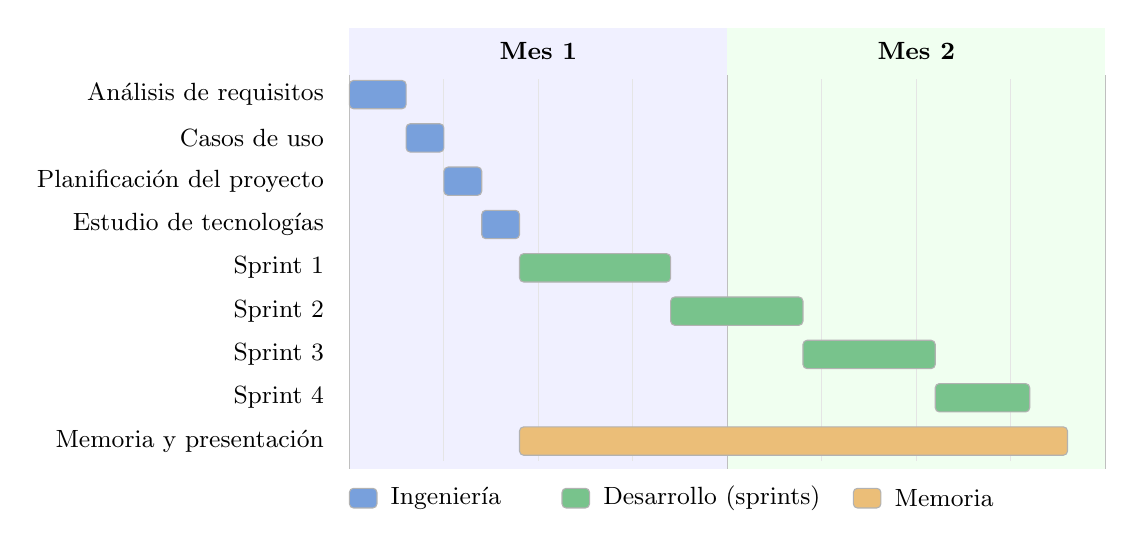
\begin{tikzpicture}[font=\small]
		% --- Parámetros: x(d) = 4.4 + 0.24*d (d en días laborables) ---
		% Bandas de meses (cada mes ~20 días laborables)
		\fill[blue!6]  (4.4,0.75) rectangle (9.2,6.35);
		\fill[green!6] (9.2,0.75) rectangle (14.0,6.35);
		\node at (6.8,6.05) {\bfseries Mes 1};
		\node at (11.6,6.05) {\bfseries Mes 2};
		% Separadores verticales de mes
		\foreach \x in {4.4,9.2,14.0} \draw[gray!50] (\x,0.75) -- (\x,5.75);
		% Líneas de rejilla por semana (cada 5 días)
		\foreach \d in {5,10,15,25,30,35} \draw[gray!20] ({4.4+0.24*\d},0.85) -- ({4.4+0.24*\d},5.7);

		% --- Filas (etiquetas) ---
		\foreach \y/\name in {%
			5.50/Análisis de requisitos,
			4.95/Casos de uso,
			4.40/Planificación del proyecto,
			3.85/Estudio de tecnologías,
			3.30/Sprint 1,
			2.75/Sprint 2,
			2.20/Sprint 3,
			1.65/Sprint 4,
			1.10/Memoria y presentación}
			\node[anchor=east] at (4.2,\y) {\name};

		% --- Barras: \fill de x(inicio) a x(fin) ---
		\definecolor{ging}{RGB}{120,160,220}
		\definecolor{gdev}{RGB}{120,195,140}
		\definecolor{gmem}{RGB}{235,190,120}
		\tikzset{bar/.style={rounded corners=1.5pt, draw=black!30}}
		\fill[bar,fill=ging] (4.40,5.32) rectangle (5.12,5.68); % 0-3
		\fill[bar,fill=ging] (5.12,4.77) rectangle (5.60,5.13); % 3-5
		\fill[bar,fill=ging] (5.60,4.22) rectangle (6.08,4.58); % 5-7
		\fill[bar,fill=ging] (6.08,3.67) rectangle (6.56,4.03); % 7-9
		\fill[bar,fill=gdev] (6.56,3.12) rectangle (8.48,3.48); % 9-17
		\fill[bar,fill=gdev] (8.48,2.57) rectangle (10.16,2.93); % 17-24
		\fill[bar,fill=gdev] (10.16,2.02) rectangle (11.84,2.38); % 24-31
		\fill[bar,fill=gdev] (11.84,1.47) rectangle (13.04,1.83); % 31-36
		\fill[bar,fill=gmem] (6.56,0.92) rectangle (13.52,1.28); % 9-38 (paralelo)

		% --- Leyenda ---
		\fill[bar,fill=ging] (4.4,0.25) rectangle (4.75,0.5); \node[anchor=west] at (4.8,0.375) {Ingeniería};
		\fill[bar,fill=gdev] (7.1,0.25) rectangle (7.45,0.5); \node[anchor=west] at (7.5,0.375) {Desarrollo (sprints)};
		\fill[bar,fill=gmem] (10.8,0.25) rectangle (11.15,0.5); \node[anchor=west] at (11.2,0.375) {Memoria};
	\end{tikzpicture}
	\caption{Diagrama de Gantt del proyecto (meses genéricos).}
	\label{fig:gantt}
\end{figure}

\section{Análisis de tecnologías disponibles}

La aplicación se divide en dos componentes principales: un \textbf{servicio de backend}, encargado
del procesamiento y análisis de las redes y de exponer los resultados a través de una API, y una
\textbf{aplicación cliente o frontend}, encargada de la interacción con el usuario y de la
visualización 3D en el navegador. Este es el punto del proyecto en el que se decide qué tecnologías
se van a utilizar; por eso en los capítulos anteriores se ha evitado citar tecnologías concretas. La
selección se ha basado en la idoneidad para el problema específico. A continuación se analizan y
comparan las tecnologías consideradas.

\subsection{Framework de backend y análisis de grafos}

El backend debe servir los datos de las redes al cliente a través de una API y utilizar bibliotecas
de análisis de grafos para el procesamiento de las matrices de adyacencia. Dado que Python dispone de
bibliotecas de análisis de grafos nativas (NetworkX~\cite{networkx}, igraph~\cite{igraph} o
graph-tool~\cite{graphtool}), elegir un \textit{framework} de backend en Python es la decisión más
eficiente, evitando la dificultad de crear servicios de intercomunicación entre lenguajes. La
tabla~\ref{tab:backend} compara las alternativas de \textit{framework} de backend consideradas.

\begin{table}[H]
	\centering
	\caption{Alternativas de backend en Python.}
	\label{tab:backend}
	\small
	\begin{tabularx}{\textwidth}{>{\raggedright\arraybackslash}p{2.0cm} >{\raggedright\arraybackslash}p{3.1cm} >{\raggedright\arraybackslash}X}
		\toprule
		\textbf{Framework} & \textbf{Arquitectura} & \textbf{Utilidad para el proyecto} \\
		\midrule
		Django & Monolítico (Full-stack, ``pilas incluidas'') &
			Incluye un ORM (mapeo objeto-relacional), un panel de administrador y un sistema de
			autenticación. Estos elementos no son imprescindibles para el núcleo de Brain Viz, el cual
			se enfoca en un servicio de datos. \\
		\addlinespace
		Flask & Micro-framework (Minimalista) &
			Para desarrollar APIs REST livianas, Flask es perfecto. Posibilita una integración simple y
			directa con librerías como NetworkX. Su filosofía minimalista posibilita construir
			únicamente lo que se necesita, lo cual es ideal para un servicio de API limitado. \\
		\addlinespace
		FastAPI & Micro-framework (Moderno, Asíncrono) &
			Proporciona un rendimiento más elevado debido a su carácter asíncrono (ASGI). Produce de
			manera automática documentación interactiva (OpenAPI/Swagger), lo que representa un beneficio
			importante para el desarrollo y la depuración de la API. \\
		\bottomrule
	\end{tabularx}
\end{table}

\textbf{Selección final:} se descarta Django por su enfoque monolítico, innecesario aquí. Entre Flask
y FastAPI se elige \textbf{Flask}~\cite{flask}, ya que permite crear una API totalmente funcional para
leer los ficheros de forma directa, procesarlos con NetworkX~\cite{networkx} y enviarlos como JSON al
frontend con la máxima sencillez.

\subsection{Framework de frontend (UI)}

El frontend es la parte con la que interactúa el usuario. Debe gestionar la visualización 3D y
controlar el estado de la aplicación. La tabla~\ref{tab:frontend} compara las alternativas
consideradas.

\begin{table}[H]
	\centering
	\caption{Alternativas de frontend.}
	\label{tab:frontend}
	\small
	\begin{tabularx}{\textwidth}{>{\raggedright\arraybackslash}p{1.9cm} >{\raggedright\arraybackslash}p{3.1cm} >{\raggedright\arraybackslash}p{3.1cm} >{\raggedright\arraybackslash}X}
		\toprule
		\textbf{Framework} & \textbf{Paradigma} & \textbf{Ecosistema} & \textbf{Integración 3D} \\
		\midrule
		React & Basado en componentes (Declarativo) &
			Enorme. Mantenido por Meta. &
			Contiene bindings que integran Three.js. \\
		\addlinespace
		Vue.js & Basado en componentes (Progresivo) &
			Grande. Impulsado por la comunidad. &
			Existen integraciones como \textit{trois}, que también integran Three.js. \\
		\addlinespace
		Angular & Framework completo (MVC, Modelo-Vista-Controlador) &
			Grande. Mantenido por Google. &
			La integración con librerías 3D es menos común o de más bajo nivel. \\
		\bottomrule
	\end{tabularx}
\end{table}

\textbf{Selección final:} se elige \textbf{React}~\cite{react}. Se descarta Angular por su rigidez, y
frente a Vue, React ofrece una ventaja decisiva gracias a su ecosistema de visualización 3D, en
concreto al \textit{binding} \textit{react-three-fiber}~\cite{r3f}, que permite desarrollar con gran
potencia el renderizado 3D usando Three.js.

\subsection{Tecnología de visualización 3D}

Para renderizar contenido 3D en el navegador existen distintas posibilidades a bajo nivel: el
elemento \textit{canvas} 2D (insuficiente para 3D acelerado), \textbf{WebGL}~\cite{webgl} ---el
estándar actual para el renderizado 3D acelerado por hardware en el navegador--- y el más reciente
\textbf{WebGPU}~\cite{webgpu}, todavía en adopción y con soporte desigual entre navegadores. Por su
madurez y compatibilidad, se opta por una solución basada en WebGL. Sobre esta base, la biblioteca de
alto nivel elegida debe ser capaz de renderizar grafos y permitir una interacción fluida para una
buena experiencia de usuario. La tabla~\ref{tab:viz3d} compara las bibliotecas y motores considerados.

\begin{table}[H]
	\centering
	\caption{Tecnologías de visualización 3D consideradas.}
	\label{tab:viz3d}
	\small
	\begin{tabularx}{\textwidth}{>{\raggedright\arraybackslash}p{2.4cm} >{\raggedright\arraybackslash}p{2.3cm} >{\raggedright\arraybackslash}p{1.7cm} >{\raggedright\arraybackslash}X}
		\toprule
		\textbf{Tecnología} & \textbf{Tipo} & \textbf{Nivel de abstracción} & \textbf{Caso de uso} \\
		\midrule
		PlayCanvas~\cite{playcanvas} & Motor de juego 3D (con editor) & Alto &
			Motor enfocado al desarrollo de videojuegos, con editor visual en la nube, pero su modelo no
			se adapta a la carga dinámica de datos. \\
		\addlinespace
		luma.gl / deck.gl~\cite{lumagl} & Framework de visualización de datos & Alto (geodatos) &
			Optimizado para la carga y visualización de grandes cantidades de datos geoespaciales, como
			mapas. No diseñado para grafos abstractos en 3D. \\
		\addlinespace
		graph.gl~\cite{graphgl} & Framework de visualización de grafos & Alto (grafos) &
			Proyecto con una comunidad pequeña y menos mantenido que el resto de alternativas. Alto
			riesgo de encontrar problemas y poca documentación. \\
		\addlinespace
		Babylon.js~\cite{babylon} & Motor de juego / framework 3D & Medio-Alto &
			Mantenido por Microsoft. Es un ``todo en uno'' muy potente y relativamente sencillo.
			Ecosistema robusto. \\
		\addlinespace
		Three.js~\cite{threejs} & Librería de renderizado 3D & Bajo &
			Es el estándar en la industria. La librería WebGL de más bajo nivel y más utilizada. Requiere
			más esfuerzo en la gestión de escena, cámaras, luces y bucle de renderizado manual. \\
		\bottomrule
	\end{tabularx}
\end{table}

\textbf{Selección final:} se descartan PlayCanvas, luma.gl y graph.gl por no ajustarse al uso de
visualización de datos 3D. La elección se encuentra entre Babylon.js y Three.js; ligada a la elección
previa de React, lo más lógico es
usar \textbf{Three.js~\cite{threejs} mediante \textit{react-three-fiber}}. Esta combinación aporta la
potencia y flexibilidad de Three.js con la facilidad de uso de React, ya que permite declarar
componentes como luces o cámaras igual que componentes de React, eliminando las dificultades del
bucle de renderizado manual y facilitando la conexión con el estado de la aplicación.

\subsection{Resumen del stack seleccionado}

La tabla~\ref{tab:stack} resume el stack tecnológico finalmente seleccionado para cada componente del
sistema.

\begin{table}[H]
	\centering
	\caption{Resumen del stack tecnológico seleccionado.}
	\label{tab:stack}
	\small
	\begin{tabularx}{\textwidth}{>{\raggedright\arraybackslash}p{2.2cm} >{\raggedright\arraybackslash}p{2.3cm} >{\raggedright\arraybackslash}p{2.9cm} >{\raggedright\arraybackslash}X}
		\toprule
		\textbf{Componente} & \textbf{Tecnología principal} & \textbf{Bibliotecas} & \textbf{Justificación} \\
		\midrule
		Backend & Python & Flask, NetworkX &
			Integración nativa para análisis de grafos, eficiencia y enfoque minimalista para APIs REST. \\
		\addlinespace
		Frontend & JavaScript & React, Three.js, react-three-fiber &
			Modelo declarativo de componentes, ecosistema líder y la mejor integración de su clase entre
			UI y renderizado 3D. \\
		\addlinespace
		Despliegue & Docker & Docker, Docker Compose &
			Garantiza la reproducibilidad del entorno y facilita la orquestación de los servicios de
			backend y frontend. \\
		\bottomrule
	\end{tabularx}
\end{table}

\section{Estimación de costes}

Para cerrar el capítulo se recopilan todos los datos calculados y se presenta la estimación de costes
final. El esfuerzo en recursos humanos se obtiene sumando, para cada tarea, el número de horas por el
salario por hora del rol encargado, tal y como detalla la tabla~\ref{tab:coste-humano}. El proyecto
tiene una duración total de 38 días laborables (unas 300 horas), periodo utilizado también para
calcular la parte proporcional de amortización de los equipos y las licencias.

\begin{table}[H]
	\centering
	\caption{Coste de los recursos humanos por tarea.}
	\label{tab:coste-humano}
	\small
	\begin{tabularx}{\textwidth}{>{\raggedright\arraybackslash}X >{\raggedright\arraybackslash}p{3.2cm} >{\centering\arraybackslash}p{1.1cm} >{\centering\arraybackslash}p{1.2cm} r}
		\toprule
		\textbf{Tarea} & \textbf{Rol} & \textbf{Días} & \textbf{Horas} & \textbf{Coste} \\
		\midrule
		Análisis de requisitos & Ingeniero de Requisitos & 3 & 24 & 430,80\,\euro{} \\
		Análisis de casos de uso & Ingeniero de Requisitos & 2 & 16 & 287,20\,\euro{} \\
		Planificación del proyecto & Analista & 2 & 16 & 258,40\,\euro{} \\
		Estudio de tecnologías & Analista & 2 & 16 & 258,40\,\euro{} \\
		Sprint 1 & Ingeniero de Software & 8 & 64 & 1.148,80\,\euro{} \\
		Sprint 2 & Programador & 7 & 56 & 818,72\,\euro{} \\
		Sprint 3 & Ingeniero de Datos & 7 & 56 & 861,28\,\euro{} \\
		Sprint 4 & Programador & 5 & 40 & 584,80\,\euro{} \\
		Redacción memoria y presentación & Analista & 2 & 16 & 258,40\,\euro{} \\
		\midrule
		\textbf{Total} & & \textbf{38} & \textbf{304} & \textbf{4.906,80\,\euro{}} \\
		\bottomrule
	\end{tabularx}
\end{table}

A este coste de personal se suman la amortización de los equipos y las licencias durante los 38 días
del proyecto y el coste de desplegar la aplicación en un servidor público durante el periodo de
validación y defensa (estimado en 6 meses). La tabla~\ref{tab:coste-total} recoge la estimación final.

\begin{table}[H]
	\centering
	\caption{Estimación de costes total del proyecto.}
	\label{tab:coste-total}
	\begin{tabularx}{0.9\textwidth}{X r}
		\toprule
		\textbf{Recursos} & \textbf{Coste} \\
		\midrule
		Recursos humanos                                         & 4.906,80\,\euro{} \\
		Recursos hardware (38 días $\times$ 0,47\,\euro{}/día)   & 17,86\,\euro{} \\
		Recursos software (38 días $\times$ 0,203\,\euro{}/día)  & 7,71\,\euro{} \\
		Despliegue en servidor público (VPS, 6 meses $\times$ 6,00\,\euro{}/mes) & 36,00\,\euro{} \\
		Otras tecnologías utilizadas (todas gratuitas)           & 0,00\,\euro{} \\
		\midrule
		\textbf{Coste total} & \textbf{4.968,37\,\euro{}} \\
		\bottomrule
	\end{tabularx}
\end{table}
